\documentclass[a4paper, 12pt, article]{memoir}

\setlength{\footmarkwidth}{0em}
\setlength{\footmarksep}{0em}
\setlength{\thanksmarkwidth}{0em}
\setlength{\thanksmarksep}{0em}

\usepackage{fontspec}
\usepackage{amsmath}
\usepackage[tracking=true, nopatch=footnote]{microtype}
\usepackage{scalefnt}
\usepackage{csquotes}
\usepackage[main=brazil]{babel}
\usepackage{wrapfig}
\usepackage{graphicx}
\usepackage{tikz} %for all basic options
\usepackage{tikz-qtree} %for simple tree syntax
\usepgflibrary{arrows} %for arrow endings
\usetikzlibrary{positioning,shapes.multipart} %for structured nodes
\usetikzlibrary{tikzmark}
\usepackage{tikz-qtree}
\usepackage{tree-dvips}
\usepackage{booktabs}
\usepackage{longtable}
\usepackage{array}
\usepackage{multirow}
\usepackage{wrapfig}
\usepackage{float}
\usepackage{colortbl}
\usepackage{pdflscape}
\usepackage{tabu}
\usepackage{threeparttable}
\usepackage{threeparttablex}
\usepackage[normalem]{ulem}
\usepackage{makecell}
\usepackage{xcolor}

\newcommand{\Bernoulli}{\text{Bernoulli}}
\newcommand{\LogNormal}{\text{LogNormal}}
\newcommand{\Normal}{\text{Normal}}
\newcommand{\Dirichlet}{\text{Dirichlet}}
\newcommand{\Exponencial}{\text{Exponencial}}
\newcommand{\logit}{\text{logit}}
\newcommand{\Dist}{\text{Dist}}
\newcommand{\Cop}{\text{Cop}}
\newcommand{\Sent}{\text{Sent}}
\newcommand{\Auth}{\text{Auth}}
\newcommand{\PoS}{\text{PoS}}
\newcommand{\Th}{\text{Th}}
\newcommand{\Dia}{\text{Dia}}
\newcommand{\abar}{\overline{\alpha}}
\newcommand{\bbar}{\overline{\beta}}
\newcommand{\bv}[1]{\beta_\text{#1}}
\newcommand{\bvi}[1]{\beta_{\text{#1}_i}}


\setmainfont{Gentium Plus}
\setmonofont[Scale=0.8]{Noto Sans}

\babelprovide[import, onchar=ids fonts letters]{ancientgreek}
\babelfont[ancientgreek]{rm}{Brill}
\babeltags{grc = ancientgreek}

\usepackage{hyperref}
\usepackage{linguex}
\setlength{\Exlabelsep}{0.5em}
\setlength{\SubExleftmargin}{1.5em}
\usepackage{paralist}
\usepackage{hyphenat}
\hyphenation{
  Κυ-ρι-α-κί-δη
  Θεσ-σα-λο-νί-κη
}

\usepackage[normalem]{ulem}
\RequirePackage{xcolor}
\definecolor{green}{RGB}{16,87,87} % rgb(16,87,87)
\definecolor{red}{RGB}{193, 11, 105} % rgb(193, 11, 105)
\definecolor{yellow}{RGB}{218,222,104} % rgb(218,222,104)
\definecolor{pink}{RGB}{243,179,145} % rgb(243,179,145)
\definecolor{blue}{RGB}{161,184,206} % rgb(161,184,206)

\RequirePackage{hyperref}%
\hypersetup{%
	colorlinks=true, % false: boxed links; true: colored links
	linkcolor=green,  % color of internal links
	citecolor=green,  % color of links to bibliography
	filecolor=green,  % color of file links
	urlcolor=green,
}

% Decorando bibliografia
\usepackage[backend=biber,
	style=./biblatex/abnt-caio, language=brazil,
	pretty, autolang=hyphen,
	pretty, repeatfields, noslsn, natbib, extrayear
]{biblatex}
\addbibresource{./biblio.bib}


\title{Repensando atração de caso em orações infinitivas do grego antigo}
\author{
  Caio B. A. Geraldes\thanks{
		Esta pesquisa foi financiada pela Fundação de Amparo à Pesquisa (Fapesp),
  bolsa de número 2021/06027-4.}
	\\\smallskip
	Universidade de São Paulo
	\\\smallskip
	<\href{mailto:caio.geraldes@usp.br}{\texttt{caio.geraldes@usp.br}}>
}
\date{1º de dezembro de 2025}

\begin{document}

\maketitle

\chapter{Introdução} % (fold)

Predicados secundários e adjuntos nominais modificando sujeitos de orações
infinitivas completivas em grego antigo costumeiramente concordam em caso com
o sujeito de seu domínio local, o qual recebe caso morfológico acusativo na
construção de \emph{Accusativus cum Infinitivo} (\emph{AcI}).
Quando o sujeito da infinitiva não é explicitamente expresso mas a oração
principal possui um objeto no dativo ou genitivo co\hyp{}referencial ao sujeito
da infinitiva, esses predicados ou adjuntos podem tanto ocorrer no acusativo ou
estarem ``atraídos'' ao caso do seu referente da oração principal.

\ex.\label{gloss:base}
\a.\label{gloss:noattr}συμβουλεύει \textbf{τῷ Ξενοφῶντι ἐλθόντα} {εἰς Δελφοὺς}
ἀνακοινῶσαι {τῷ θεῷ} {περὶ τῆς πορείας}.\\
Ele aconselha Xenofonte ir a Delfos e interrogar ao deus sobre a viagem.
(Xen.\ \emph{Anab.} 3.1.5)
\b.\label{gloss:attr}ἀφῆκε \textbf{μοι ἐλθόντι} {πρὸς ὑμᾶς} λέγειν τἀληθῆ.\\
Ele me permitiu ir e dizer as verdades frente a vós.
(Xen.\ \emph{Hell.} 6.1.13)

Na literatura sobre o tópico de atração de caso, foram propostas listas de
contextos em que a atração ocorre, entre os filólogos, e algumas propostas
estruturais que permitiriam a ocorrência do fenômeno, entre os gerativistas e
minimalistas.
Os fatores que influenciam na decisão do falante por alguma das resoluções
em~\ref{gloss:base} permanecem, no entanto, desconhecidos.

Em pesquisas prévias, busquei apresentar padrões distributivos que favorecem a
resolução \emph{com} atração,~\ref{gloss:attr}, mostrando haver forte associação
estatística entre atração e: 1. classe do verbo matricial, 2. classe do verbo
infinitivo, 3. distância relativa entre controlador e alvo da atração.
Argumentei, na ocasião, que esses fatores eram \emph{proxies} de valores não
anotados dos dados, como traços semânticos e pragmáticos do contexto discursivo.

Esses resultados -- e os métodos empregados para obtê-los --, no entanto, não
me pareciam satisfatórios para sustentar os resultados.
Havia ainda a possibilidade de que os fatores analisados terem interações entre
si, as quais os métodos estatísticos empregados não eram capazes de capturar e
isolar, ao menos não com os dados disponíveis.
Um segundo motivo para desconfianças sempre deve rondar pesquisas quantitativas,
o clássico adágio ``correlação não é causação''.

Hoje apresento sobretudo a solução metodológica para essas questões.
Ela virá na forma de modelos de inferência causal, desenhados para determinar
\emph{quais} correlações podem ser estimadas a partir de dados, e modelos de
regressão linear generalizada.

Os dados utilizados no que segue representam 340 sentenças extraídas do
\emph{corpus} literário ático e de Heródoto, anotados manual e
computacionalmente.


Começo pela produção de um modelo causal passo a passo.

\chapter{Natureza da atração} % (fold)

A descrição mais abstrata possível para a atração de caso em infinitivas é
quando dois constituintes, um controlador e um alvo, produzidos em diferentes
domínios de uma sentença, um dos domínios subordinando o outro, covariam na
propriedade $[Caso]$.
Essa descrição satisfaz a definição de concordância dada
por~\textcite[4--7]{Corbett2006} em seu estudo tipológico sobre concordância em
línguas naturais.

A falta de covariação de $[Caso]$ é, via de regra, considerada um resultado da
aplicação das regras padrão de concordância nominal em grego antigo, conquanto
se considere que todos os sujeitos de orações infinitivas recebem caso
\emph{acusativo} e que sujeitos não explicitamente produzidos são marcados para
a propriedade $[Caso]$ podem controlar concordância.
A regra padrão de concordância nominal poderia ser expressa por algo como:
``dois constituintes nominais co\hyp{}referenciais concordam em caso quando
pertencentes ao mesmo domínio sintático''.

Os fatos de, em casos nos quais a atração de caso é uma opção de
concordância, haver opção de controlador para o alvo (ou o objeto oblíquo da
principal ou o sujeito implícito da infinitiva), $[Caso]$ ser uma propriedade
não\hyp{}lexical e o domínio ser não\hyp{}local (i.e. transoracional) favorecem
a interpretação de que o tipo de concordância observado na atração de caso é
menos canônico do que as demais resoluções de concordância em grego antigo,
seguindo os critérios do mesmo~\textcite[pp. 8ff.]{Corbett2006}.

Se tal é o caso, espera-se que a atração se comporte como exemplos tipos de
concordância não\hyp{}canônica em línguas naturais e que a opção menos canônica
tenderá a ser condicionada por fatores semelhantes aos que as condicionam.
Propriedades do controlador, domínio e alvo da concordância são os
principais condicionantes da escolha entre uma resolução canônica e
não\hyp{}canônica de concordância.
Um modelo do tipo pode ser representado utilizando o grafo direcionado acíclico
assim, em que
\textbf{A}tração ($\simeq$ Concordância) é \emph{causada}
pelo \textbf{C}ontrolador, \textbf{D}omínio e \textbf{Al}vo:

\begin{wrapfigure}{o}{0.5\textwidth}
  \begin{center}
    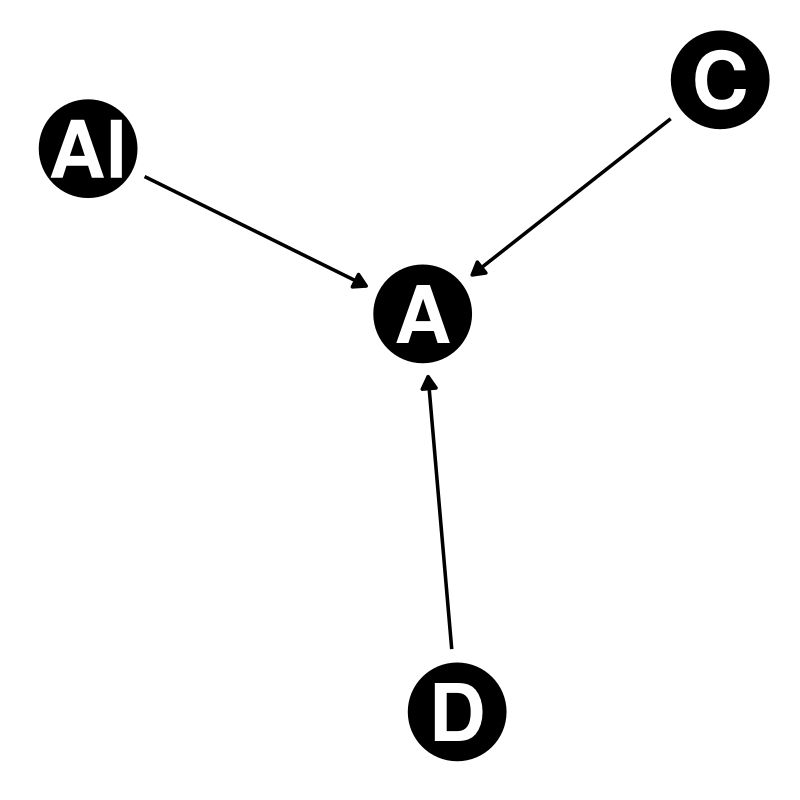
\includegraphics[width=0.41\textwidth]{./plots/dag_non_canonical_agreement.png}
  \end{center}
\end{wrapfigure}

Esses nódulos representam conjuntos de fatores linguísticos, alguns que podem
ser observados diretamente (classe de palava do alvo), alguns podem ser intuídos
(animacidade) e outros podem ser inobserváveis (função discursiva, dado que grego
não marca focos e tópicos na morfossintaxe de maneira regular).
Quando um fatos observado for incluído ao modelo a seguir, dividirei o nódulo
em dois: um contendo o novo fator observável e um contendo o resto dos fatores
não observados.

% chapter Nature of attraction (end)

\chapter{Domínio da atração} % (fold)

\textcite{KG} e outros associaram a atração de caso a sentenças em que a oração
infinitiva é tem um verbo copular como εἶναι ou γενέσθαι, mas também φαίνεσθαι.
Há motivos para que a classe do infinitivo favoreça uma opção de concordância ou
outra?
Diretamente elas podem delimitar o tipo de relação entre controlador e alvo:
quando estão presentes, a relação mais provável é aquela de predicação primária,
ao invés de predicação secundária ou apositiva.
Não obstante, estamos interessados também na interação entre variáveis que afetem
a atração de caso, e infinitivos copulares podem influenciar também
indiretamente a atração de caso por selecionarem a opção de classe de palavras:
substantivos e adjetivos se tornam especialmente mais prováveis que particípios
quando o verbo de uma oração é copular, já que estamos atribuindo uma
propriedade, uma identidade ou pertencimento a uma classe, os três denotados por
adjetivos e substantivos.

Sabe-se que esses fatores, classe da relação entre termos e classe de palavras,
afetam a seleção de concordância e duas hierarquias já foram propostas para
prever quando a resolução menos canônica (também chamada de concordância
semântica) é mais provável, a Hierarquia de Concordância~\cite{Corbett1979} e
Hierarquia de Predicados~\cite{Comrie1975}, combinadas
em~\ref{hierar:agreementpredicate2}:


\ex.\label{hierar:agreementpredicate2} Hierarquias de Predicados e Concordância~\citep[233]{Corbett2006}:\\
\begin{tikzpicture}[baseline=0pt]
  \node (attr) at (0, 0) {Atributivo};
  \node (pred) at (2.5, 0) {Predicado};
  \node (predv) at (2.9, -0.4) {Verbal};
  \node (predp) at (3.5, 1) {Participal};
  \node (preda) at (5, 2) {Adjetival};
  \node (predn) at (7.5, 2.7) {Substantival};
  \node (relp) at (5.6, 0) {Pronome relativo};
  \node (perp) at (9.1, 0) {Pronome pessoal};
  \node (less) at (0, -1) {-};
  \node (plus) at (9.1, -1) {+};
  \draw[->, thick] (attr) to (pred);
  \draw[->, thick] (pred) to (relp);
  \draw[->, thick] (relp) to (perp);
  \draw[->, thick] (pred) to (predp);
  \draw[->, thick] (predp) to (preda);
  \draw[->, thick] (preda) to (predn);
  \draw[->] (less) to (plus);
  \draw[->] (plus) to (less);
  \node at (4.5, -1.5) {Probabilidade de concordância por justificativa
    semântica};
\end{tikzpicture}


Incluindo essas associações ao modelo causal, dizemos que
\textbf{A}tração é causada pela relação \textbf{c}opular ou não entre
controlador e alvo e pela classe de palavra (\textbf{PoS}), a qual também é
``causada'' pela classe de relação entre controlador e alvo, bem como por outros
efeitos não observados do domínio e alvo.
Aplicando o \emph{do-calculus}~\cite{Pearl2009}, sabemos que o efeito direto da classe
de palavra requer ajustar o modelo estatístico por $Cop$, para bloquear o
caminho não causal
$PoS \leftarrow Cop  \rightarrow A$.

\begin{center}
  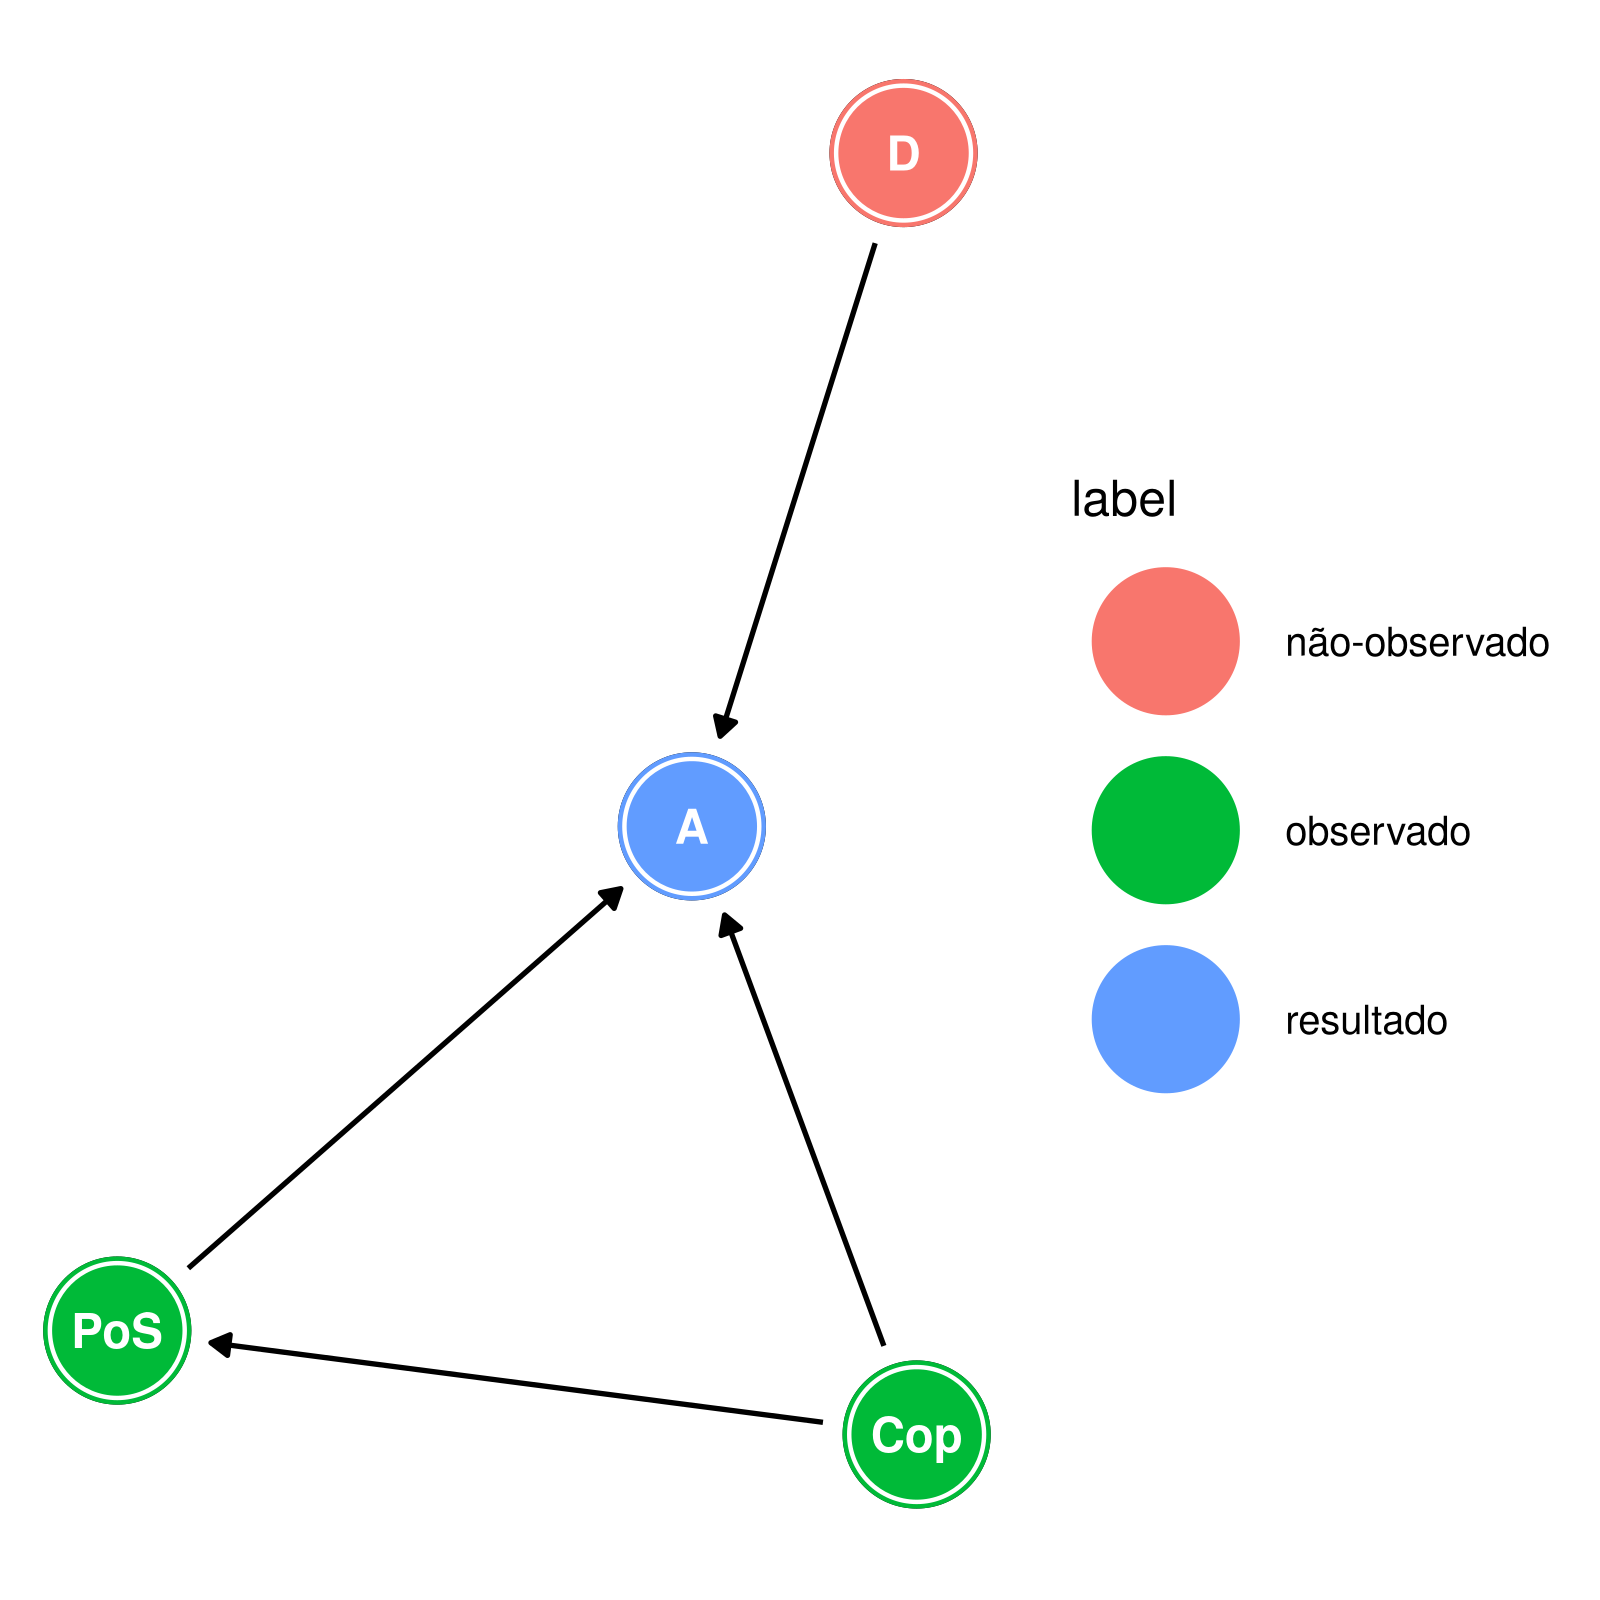
\includegraphics[width=0.4\linewidth]{./plots/dag_a.png}
\end{center}

\chapter{Controlador da atração}

Outra associação por vezes proposta na literatura é aquela entre atração de caso
e verbos principais impessoais.
No entanto, em trabalhos prévios, demonstrei que essa
associação não existe para todos os verbos impessoais em que a atração de caso é
possível, que a forma impessoal do verbo δοκέω `parecer melhor' praticamente
nunca apresenta atração de caso e que os verbos impessoais que de fato possuem
associação estatística com a ocorrência de atração de caso são aqueles que
possuem semântica modalizadora, como ἔξεστί `ser possível' e ἐξαρκεῖ `ser
suficiente'.


Não há motivos linguísticos para que a classe do verbo principal afete
diretamente a concordância entre controlador e alvo.
Entretanto, é plausível que ela interfira indiretamente, ao selecionar
propriedades do controlador da atração de caso.
Verbos de semântica modalizadora carregam pouquíssima informação
semântica, de modo que o papel temático de seu objeto indireto depende
integralmente do verbo infinitivo.
σοι em~\Next{} age como uma espécie de \emph{quirk subject} e tem o papel
temático de agente.
Isso contrasta muito com exemplos em que a sentença é construída com verbos de
ordem e conselho, como συμβουλέυω `aconselhar', cujo
objeto indireto é um recipiente da ação, e com aqueles em que a sentença é
construída com o verbo δοκεῖ `parecer melhor', cujo
objeto indireto representa um experienciador, `aquele a quem X parece ser melhor
ser feito'.

\ex. Ἀλλ᾽ ἐξαρκῇ σοι τὰ ἔργα αὐτῶν ὁρῶντι σέβεσθαι καὶ τιμᾶν τοὺς θεούς.\\
Mas será suficiente a ti ver esses feitos e respeitar os deuses.
(Xen.\ Mem. 4.3.13)

Isso, no entanto, apenas vale se o verbo infinitivo não for uma cópula, caso o
contrário, o papel temático será algo próximo ao de um experienciador, o que
significa que o papel temático \textbf{Th} é um nódulo irmão de \textbf{PoS},
causado por \textbf{Cop}.
Incluindo ao DAG, temos o modelo:

\begin{center}
  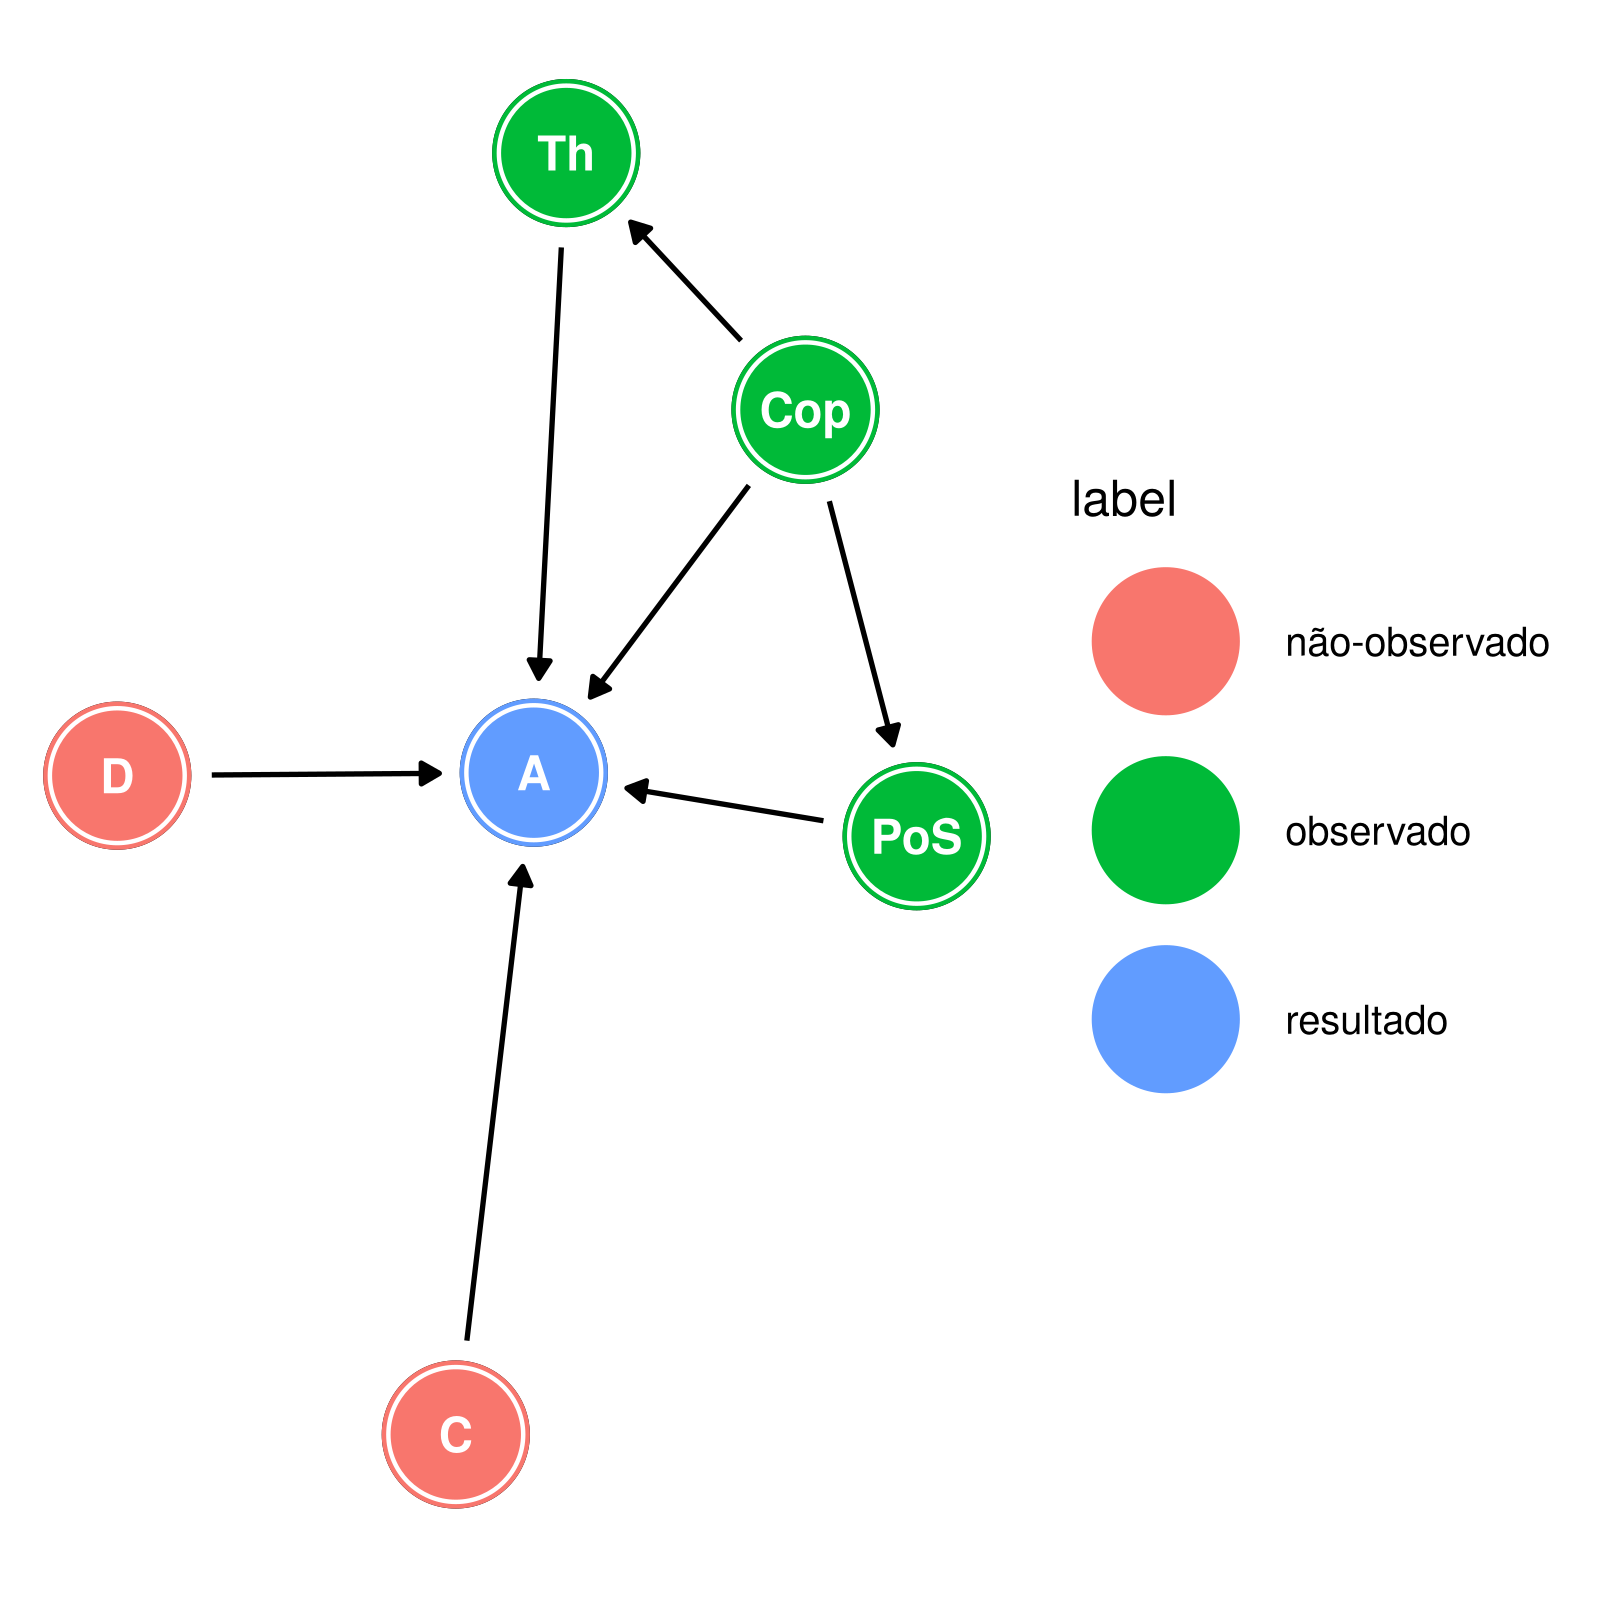
\includegraphics[width=0.4\linewidth]{./plots/dag_b.png}
\end{center}

\chapter{Intermezzo: autoria, gêneros literários e dialetos}

% TODO: incluir referências
É prática comum na linguística de línguas clássicas (grego e
latim) controlar a distribuição de fenômenos linguísticos pela autoria atribuída
ao documento fonte.
Do ponto de vista causal, a inclusão deste controle representa a pressuposição
teórica de que traços particulares de cada autor -- seja de sua posição social,
ou de suas idiossincrasias de estilo -- têm efeito direto na probabilidade de
uma certa forma linguística ser atestada ou não.
O mesmo costuma ser feito com gêneros literários, sob o pressuposto de que
certas convenções de gênero favoreceriam certas construções linguísticas.
Essa prática, no entanto, corre o risco de produzir associações estatísticas
espúrias se não for avaliado cuidadosamente o modelo causal pressuposto para o
fenômeno.

Como argumentei anteriormente, verbos
de semântica modalizadora, e por conseguinte certos papéis temáticos atribuídos
aos objetos oblíquos nas sentenças com possibilidade para atração de caso, são
preferidos em textos do gênero do diálogo filosófico em contraste ao gênero
historiográfico, dado que o primeiro teria, pela natureza de seu assunto,
mais motivos para produzir predicados deônticos ou sobre a possibilidade de
certos eventos enquanto o último teria mais motivos para expor cenas de
conselho e ordem, dado que preocupado com eventos militares.

Assim, o uso de certos verbos é condicionado pela escolha de um gênero
literário ou tema de escrita pelo autor.
Além do efeito direto entre \textbf{Aut}oria e uso da atração de caso, há um caminho
indireto que passa por sua escolha de gênero literário, a consequente tendência
de um certo tema usar verbos que selecionam diferentes papeis temáticos em
orações com a possibilidade de atração que, por fim, consideramos poder afetar
a probabilidade de atração de caso.
Adicionamos assim \textbf{Aut}oria, \textbf{G}ênero e \textbf{Dia}leto ao
DAG:

\begin{center}
  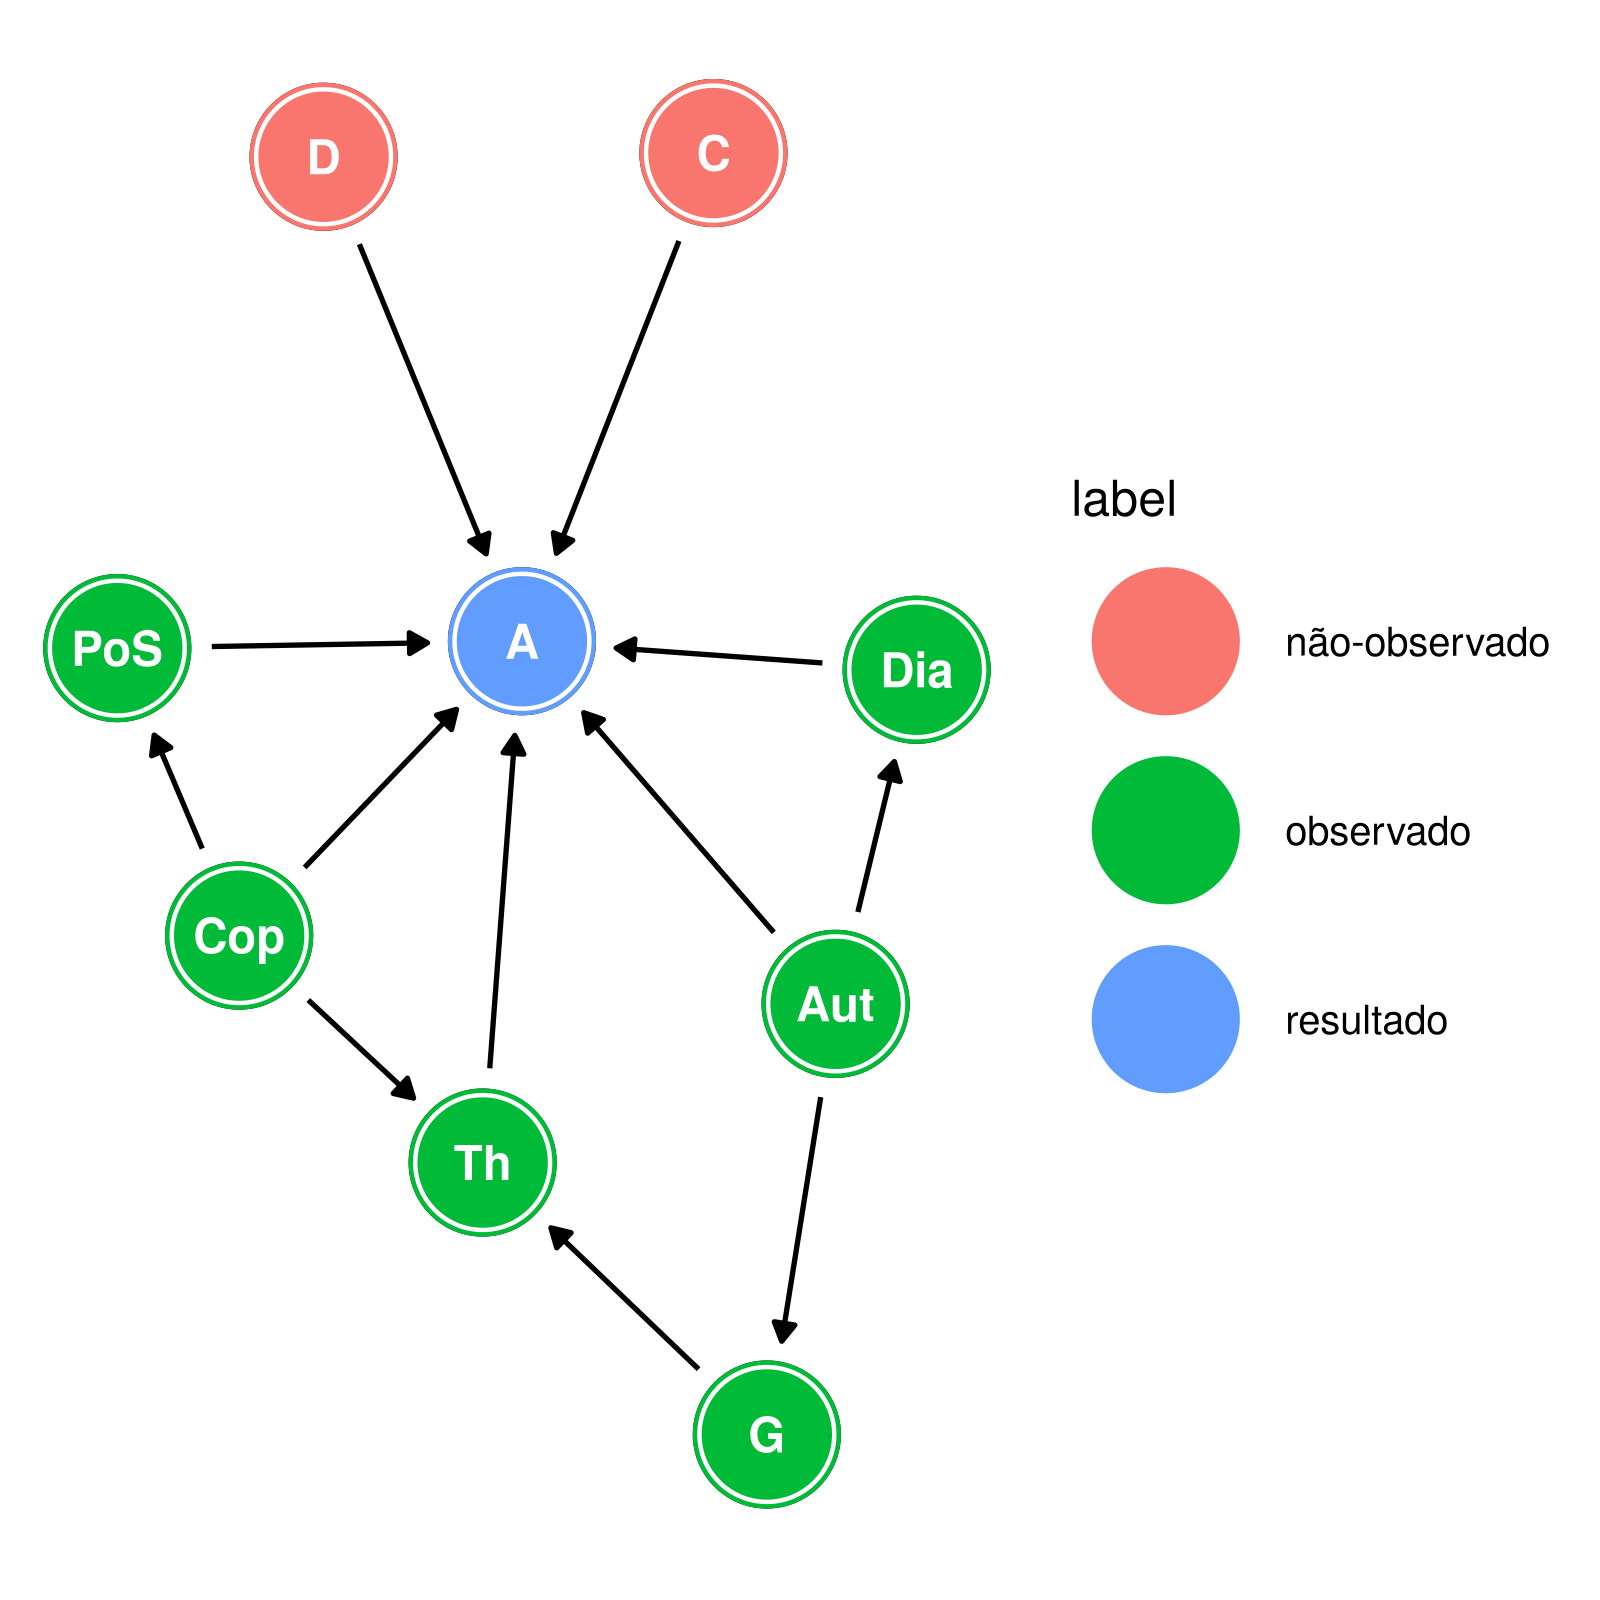
\includegraphics[width=0.4\linewidth]{./plots/dag_c.png}
\end{center}

Estas adições tem as seguintes consequências a partir do \emph{do-calculus}:
\begin{compactitem}
  \item para estimar o efeito direto de \textbf{Th}, deve-se controlar por
        \textbf{Cop}ula e ou por \textbf{G}ênero ou por \textbf{Aut}oria;
  \item para estimar o efeito direto de \textbf{Cóp}ula, deve-se controlar por
        \textbf{PoS}, \textbf{Th}, e ou por \textbf{G}ênero ou por \textbf{Aut}oria;
  \item para estimar o efeito direto de \textbf{Aut}oria,  deve-se controlar ou
        por \textbf{G}ênero ou \textbf{Cop}ula e \textbf{Th}.
\end{compactitem}


\chapter{Alvo da atração}

Uma última associação que há muito é proposta é que a atração é mais provável
quando controlador e alvo estão \emph{próximos} um do outro e que conforme a
distância aumenta, manos provável é a atração de caso.
Além disso, os dados mostram que em todos os casos de
precedência do alvo com relação ao controlador, como no
exemplo~\ref{ex:hosagathois}, onde, do ponto de vista da função comunicativa,
ἀγαθοῖς funciona como foco.

  {
    \SingleSpacing%
    \ex.\label{ex:hosagathois}\textbf{ἀγαθοῖς} τε \textbf{ὑμῖν} προσήκει εἶναι.\\
    Boa gente é o que vos é dado ser. (Xen.\ Anab. 3.2.11)

  }

Não se pode, no entanto, anotar os dados para função comunicativa de maneira
confiável, livre de interpretações \emph{ad hoc} e reprodutível em grego antigo,
dado que a língua não emprega regularmente expedientes morfológicos ou lexicais
para marcar a função comunicativa dos sintagmas.
Mesmo que ordem de palavras seja um bom previsor de função comunicativa em
grego, não é possível produzir uma relação $1:1$ a partir dela.

Para nossa modelagem causal o que importa é que, partindo do pressuposto que
informações pragmáticas codificadas no alvo produzem efeitos na probabilidade de
atração de caso, haveria uma associação indireta e espúria entre ordem de
palavras $OP$ e atração, pois ambas seriam nódulos filhos de $Al$.
Ainda que se julgue que $OP$ tem efeito direto sobre $A$, isto é, que a
precedência do alvo com relação ao controlador \emph{causa} atração de caso,
ainda assim seria impossível, sem controlar por $Al$, estimar o efeito causal
$OP \rightarrow{} A$.
Isso faz da ordem de palavras um efeito impossível de estimar sem enviesamento
com os dados disponíveis, a não ser que seja encontrado um meio de anotar com
precisão os valores pragmáticos do alvo.
O DAG final é então:

\begin{center}
  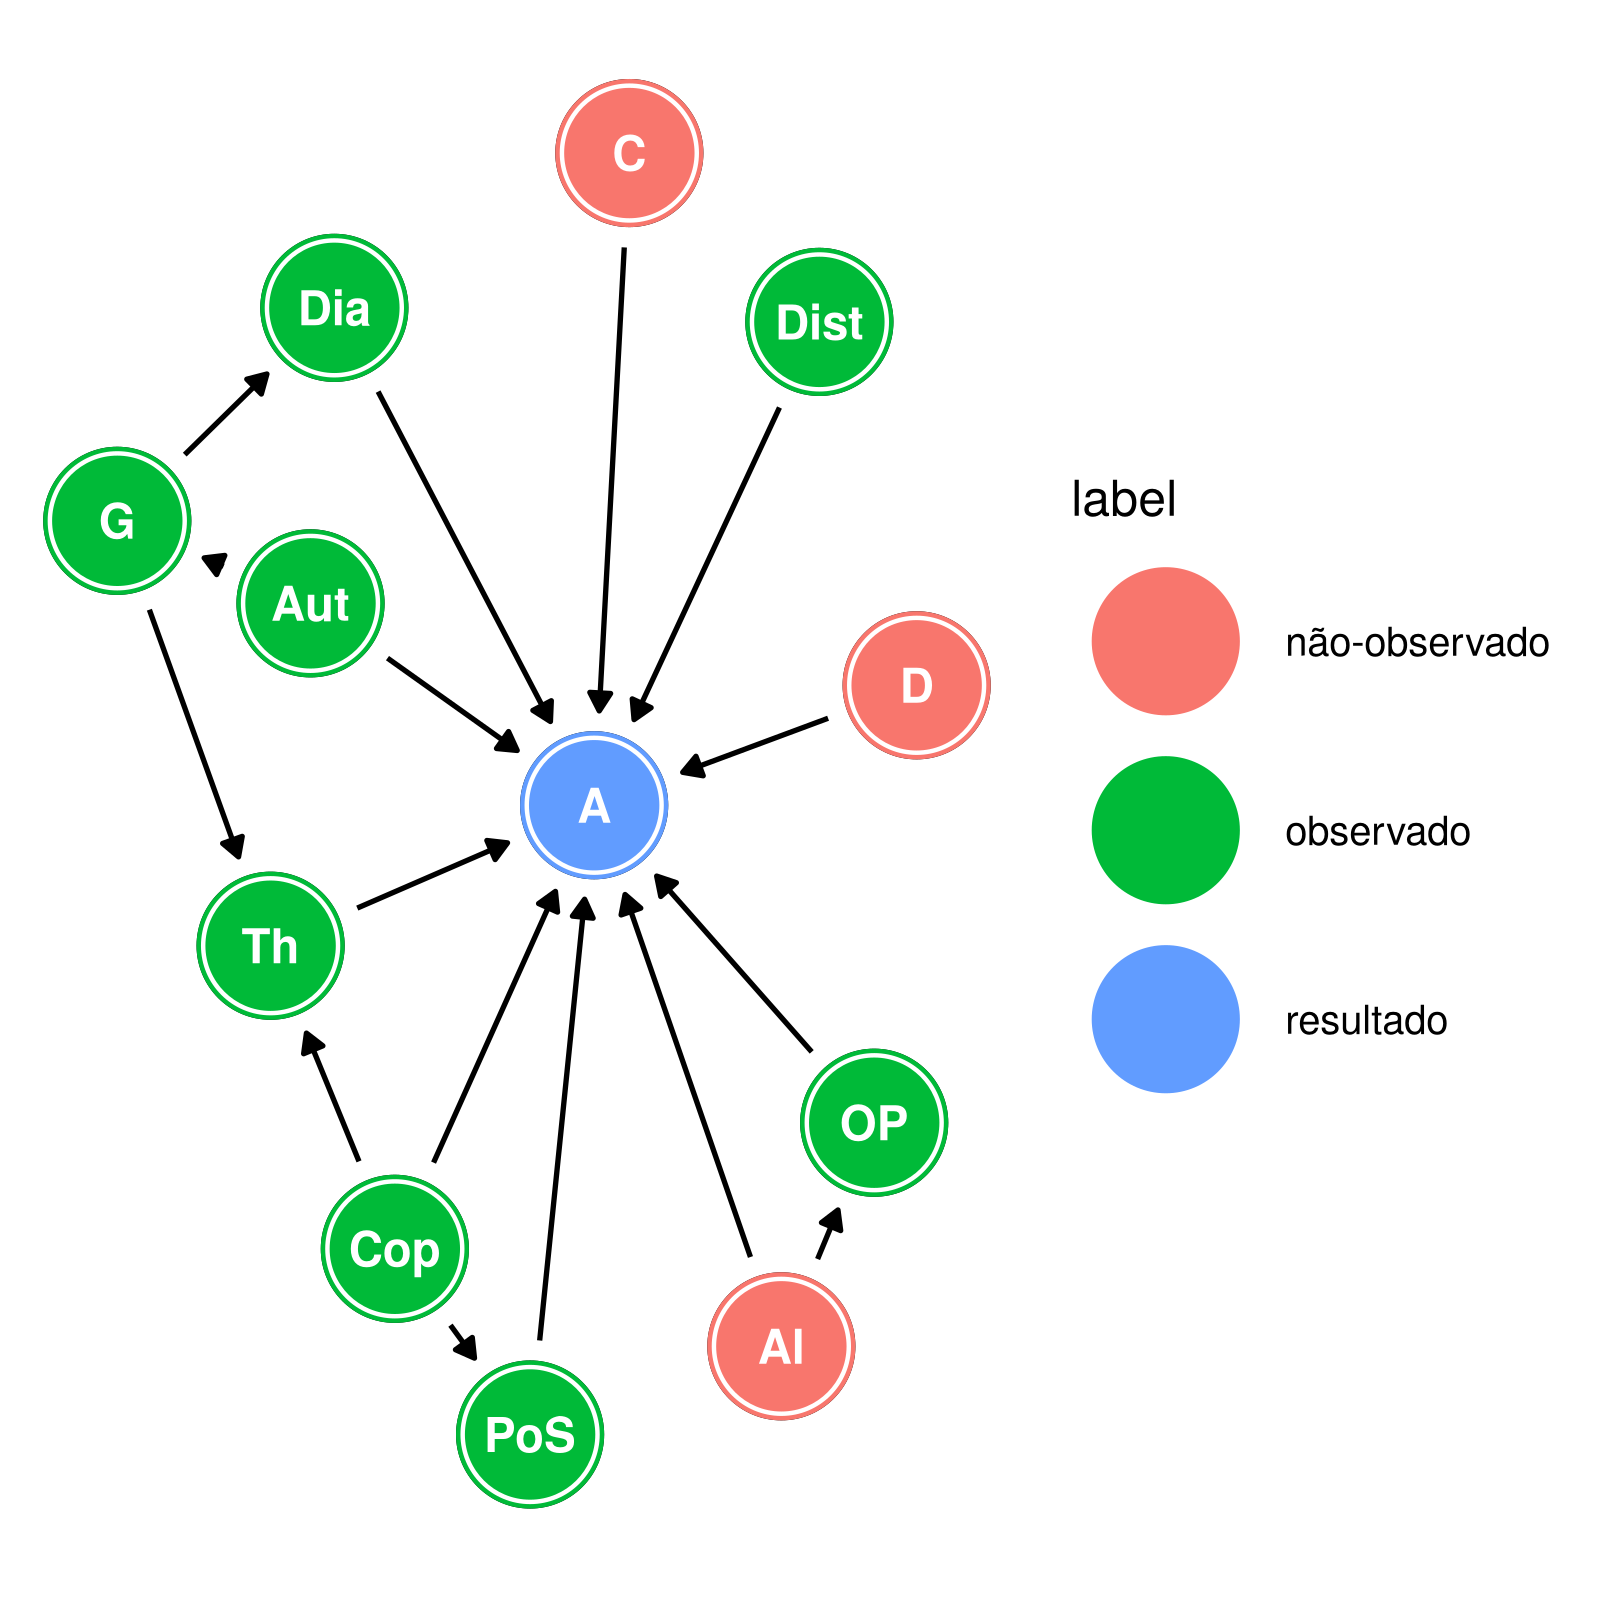
\includegraphics[width=0.4\linewidth]{./plots/dag_d.png}
\end{center}


\chapter{Análise} % (fold)

Não são necessários diversos modelos para estimar os efeitos da maioria dos
fatores de interesse.
Pela aplicação do \emph{do-calculus},
ordem de palavras, pode-se estimar o efeito direto de:
\begin{inparaenum}
  \item classe gramatical do alvo;
  \item classe de predicação do domínio;
  \item papel temático do controlador;
  \item dialeto;
  \item autoria; e
  \item distância entre controlador e alvo.
\end{inparaenum}
Para remover informação da ordem de palavras, deve-se utilizar o valor absoluto
da distância, de modo que antecedência não esteja codificada nos dados.
Com isso, temos o seguinte modelo linear:

\begin{align*}
  \text{A}                                                & \sim \Bernoulli(p_i)                                                                                       \\
  \logit(p_i)                                             & = \alpha_{\Sent} + \bv{Cop}\Cop_i + \bv{Dist}|\Dist_i| +                                                   \\
                                                          & + \bv{PoS}\sum^{\PoS_{i}-1}_{j=0}{\delta_{j_{\PoS}}}      + \bv{Th}\sum^{Th_{i}-1}_{j=0}{\delta_{j_{\Th}}} \\
                                                          & + \bvi{Auth} + \bvi{Dia}                                                                                   \\
  \alpha                                                  & = \abar_\Sent + z_{\Sent} * \sigma_\Sent                                                                   \\
  \bv{Cop}, \bv{Dist}                                     & \sim \Normal(0, 1)                                                                                         \\
  \bv{PoS}, \bv{Th}                                       & \sim \Normal(0, 1)                                                                                         \\
  \delta_{\PoS}, \delta_{\Th}                             & \sim \Dirichlet(2)                                                                                         \\
  \bv{Auth}                                               & = z_{\Auth}*\sigma_{\Auth}                                                                                 \\
  \bv{Dia}                                                & = \bbar_\Dia + z_{\Dia}*\sigma_{\Dia}                                                                      \\
  \abar_\Sent, \bbar_\Dia, z_{\Sent}, z_{\Auth}, z_{\Dia} & \sim \Normal(0,1)                                                                                          \\
  \sigma_{\Sent}, \sigma_{\Auth}, \sigma_{\Dia}           & \sim \Exponencial(1)
\end{align*}

Essa monstruosidade apenas serve de máquina para estimar a magnitude relativa
dos efeitos $\beta$ na probabilidade $p$ de atração de caso dado o valor de cada
variável ($\Cop$, $\PoS$ etc).
Dela dois detalhes merecem mais atenção:
Os \emph{priors} são bastante ``planos'', e representam com isso a incerteza que
temos sobre qual a verdadeira magnitude do efeito das variáveis: a equação só
sabe que sabemos muito pouco.
Os efeitos de $\bv{PoS}$ e $\bv{Th}$ é estimado usando essas somas mais
chamativas, porque decidi modelar estes efeitos como o de preditores categoriais
ordenados.
Os efeitos de classe gramatical $PoS$ e papel temático $Th$ são modelados como
Preditores Categóricos Ordenados utilizando uma distribuição Dirichlet.
Isso é feito parar representar a ideia geralmente aceita de que hierarquias
tipológicas como a Hierarquia de Concordância~\cite{Corbett1979} e Hierarquia de
Predicados~\cite{Comrie1975} em~\ref{hierar:agreementpredicate2} tem pontos ``de
corte'' entre seus nódulos e que o seu efeito aumenta de maneira monotônica
através deles.
O primeiro nódulo de cada hierarquia tem o efeito base $0$, e os nódulos
seguintes acumulam parte do efeito total $b_X$.

Os efeitos de autoria ($\beta_\text{Auth}$) e dialeto ($\beta_\text{Dia}$),
bem como a medida do efeito de fatores não observados das sentenças
($\alpha_\text{Sent}$) foram representados por priors não centralizados
para realizar \emph{partial pooling}, a fim de que seja possível estimar quanta
variação o modelo observa entre os autores, dialetos e sentenças e permitir
posterior expansão do modelo para outros dialetos.

\section{Cópula e distância} % (fold)

Os fatores mais associados pela literatura, cópula e distância, mostram os
resultados esperados:

\begin{center}
  
\begin{tabular}[t]{lrrrrr}
\toprule
Effect & mean & sd & 5.5\% & 94.5\% & rhat\\
\midrule
$\beta_{\text{Copula}}$ & 1.81 & 0.47 & 1.07 & 2.57 & 1.00\\
$\beta_{\text{Dist}}$ & -0.27 & 0.06 & -0.37 & -0.18 & 1.01\\
\bottomrule
\end{tabular}

\end{center}

\begin{figure}[!h]
  \centering
  \begin{minipage}{.48\textwidth}
    \centering
    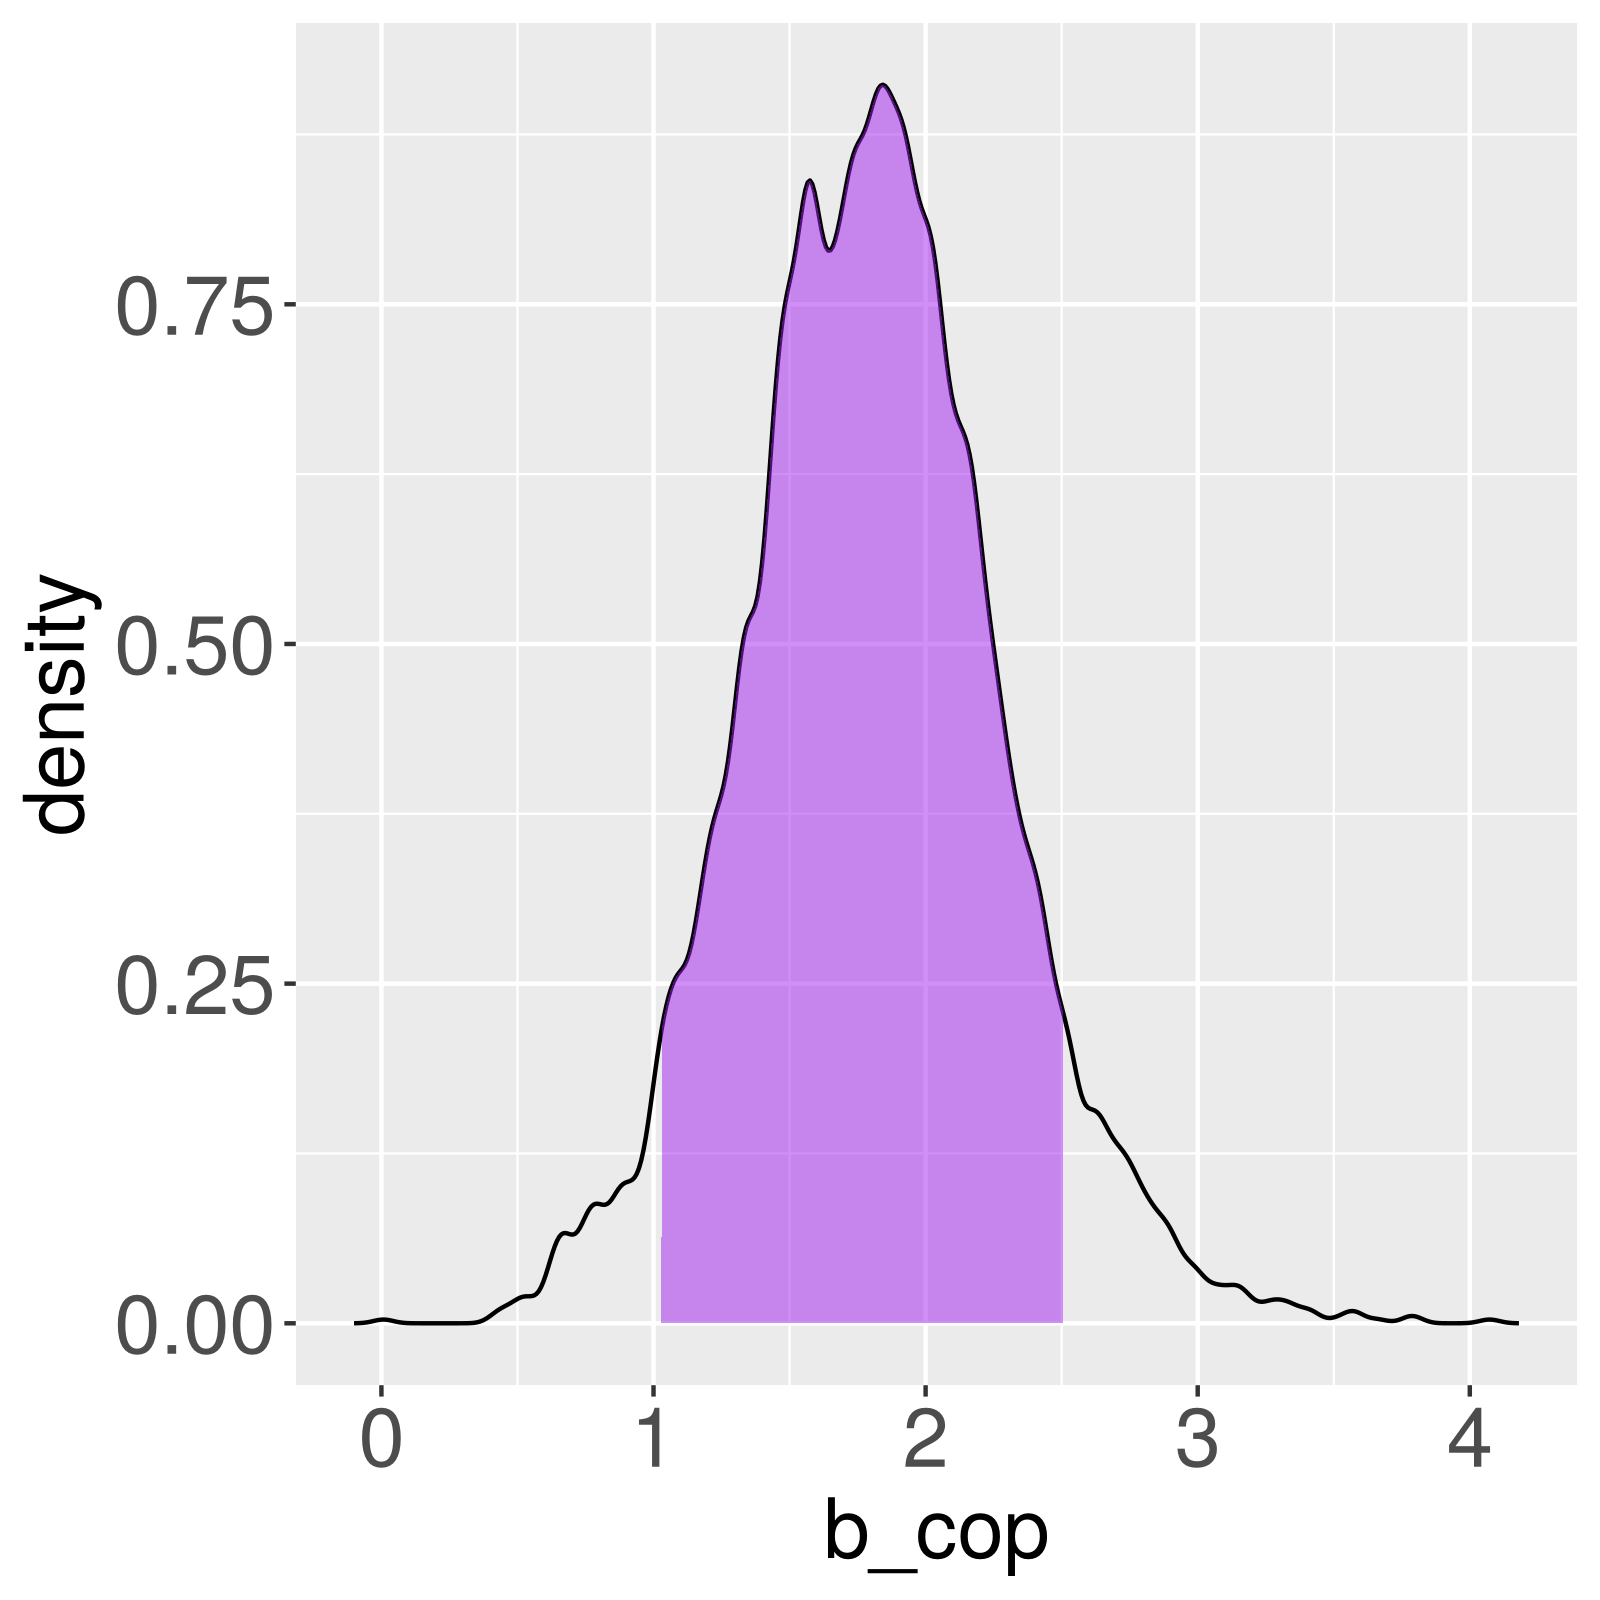
\includegraphics[width=\linewidth]{./plots/posterior_b_copula.png}
  \end{minipage}%
  \hfill
  \begin{minipage}{.48\textwidth}
    \centering
    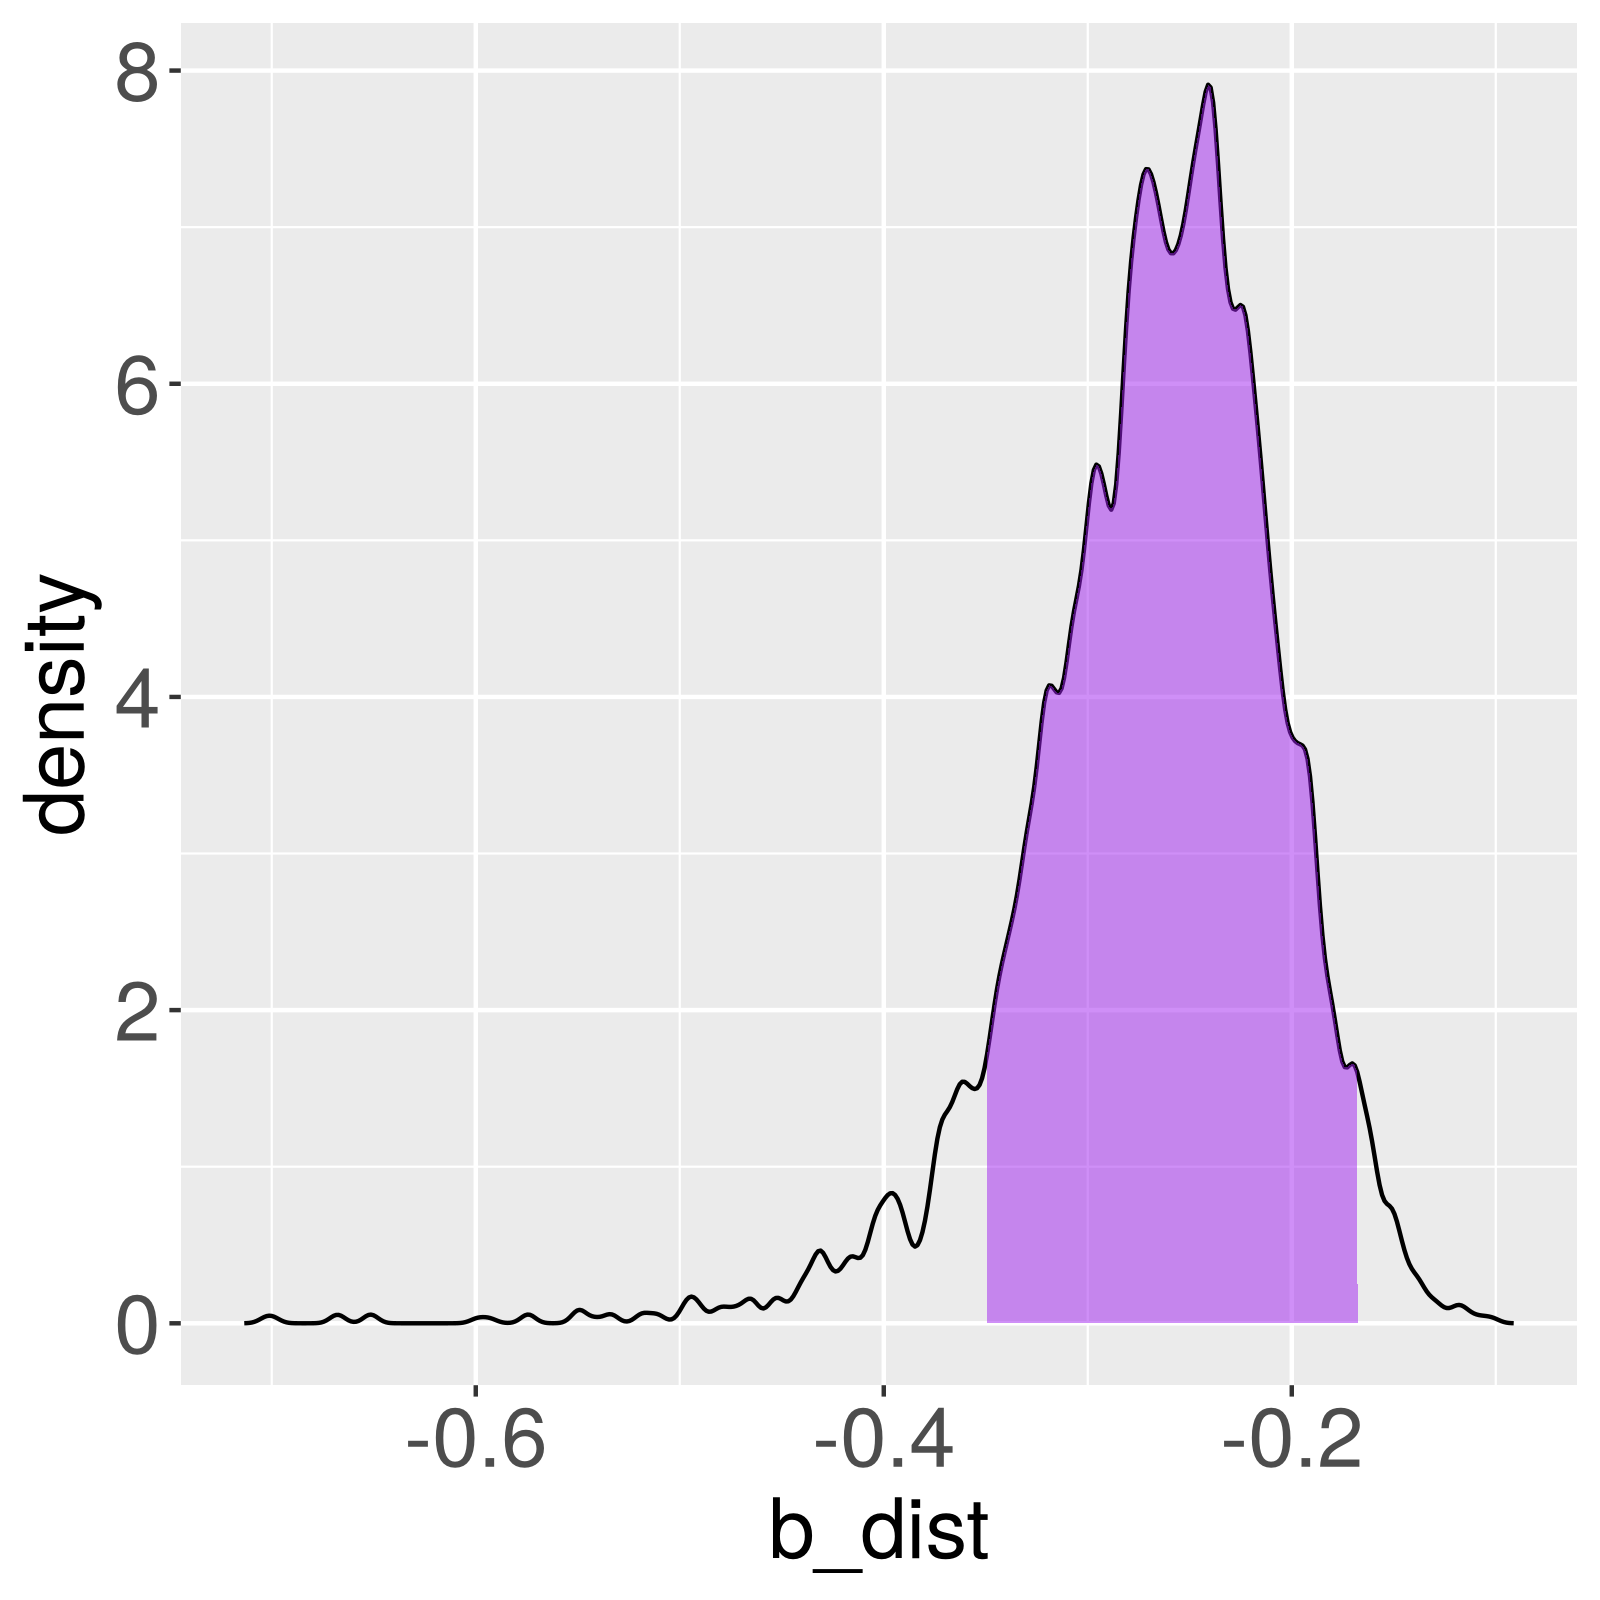
\includegraphics[width=\linewidth]{./plots/posterior_b_dist.png}
  \end{minipage}
\end{figure}

Note que o efeito de distância é bastante preciso.
Para oferecer uma intuição de seu significado, suponha que uma sentença $X$, com
verbo infinitivo copular seja produzida repetidas vezes exatamente da mesma
maneira em conteúdo e forma, apenas aumentando a distância entre controlador e
alvo.
Uma vez que a distância chegasse a 8 palavras, qualquer efeito do
infinitivo ser copular sobre a probabilidade da atração de caso seria negado
Se nosso modelo causal estiver correto, esse é um resultado importante do ponto
de vista tipológico, posto que a evidência em outras línguas sugere que o
aumento da distância entre controlador e alvo favoreça a concordância não
canônica, enquanto aqui temos precisamente o oposto.

% section Copula and Distance (end)

\section{Classe de palavras e hierarquia de predicado} % (fold)

Em palavras, o modelo prevê que é há um efeito considerável da classe de
palavras do alvo e a probabilidade atração e o efeito aumenta de maneira
aproximadamente monotônica conforme o alvo se torna mais canonicamente
``nominal''.
Há ainda bastante incerteza na magnitude do efeito.

\begin{center}
  
\begin{tabular}[t]{lrrrrr}
\toprule
Effect & mean & sd & 5.5\% & 94.5\% & rhat\\
\midrule
$\beta_{\text{PoS}}$ & 0.76 & 0.51 & 0.17 & 1.71 & 1\\
$\delta_{\text{Adj}}$ & 0.48 & 0.18 & 0.19 & 0.78 & 1\\
$\delta_{\text{Noun}}$ & 0.52 & 0.18 & 0.22 & 0.81 & 1\\
\bottomrule
\end{tabular}

  \bigskip
  
\begin{tabular}[t]{llrrrrr}
\toprule
PoS & Cummulative effect & mean & sd & 5.5\% & 94.5\% & rhat\\
\midrule
Participle & $\beta_{\text{PoS}} * 0$ & 0.00 & 0.00 & 0.00 & 0.00 & --\\
Adjective & $\beta_{\text{PoS}} * \delta_{\text{Adj}}$ & 0.35 & 0.26 & 0.06 & 0.86 & 1\\
Noun & $\beta_{\text{PoS}} * (\delta_{\text{Adj}} + \delta_{\text{Noun}})$ & 0.76 & 0.51 & 0.17 & 1.71 & 1\\
\bottomrule
\end{tabular}

\end{center}


\section{Papel temático do controlador} % (fold)

Aqui a estimativa é levemente mais precisa e notoriamente mais forte.
Quanto mais canonicamente ``sujeito'' for o papel temático atribuído ao
controlador, tanto mais provável é a atração de caso.
Esse é o maior efeito observado e, mesmo com a incerteza grande (desvio padrão
de 0.6), o efeito é grande e positivo: agentes mais que duplicam a probabilidade
de atração de casa em comparação ao experienciadores e a quadruplicam em relação
a recipientes.

\begin{center}
  
\begin{tabular}[t]{lrrrrr}
\toprule
Effect & mean & sd & 5.5\% & 94.5\% & rhat\\
\midrule
$\beta_{\text{Theta}}$ & 2.73 & 0.60 & 1.88 & 3.76 & 1\\
$\delta_{\text{Exp}}$ & 0.38 & 0.12 & 0.19 & 0.57 & 1\\
$\delta_{\text{Agent}}$ & 0.62 & 0.12 & 0.43 & 0.81 & 1\\
\bottomrule
\end{tabular}

  \bigskip
  
\begin{tabular}[t]{llrrrrr}
\toprule
Theta & Cummulative effect & mean & sd & 5.5\% & 94.5\% & rhat\\
\midrule
Recipient & $\beta_{\text{Th}} * 0$ & 0.00 & 0.00 & 0.00 & 0.00 & --\\
Experiencer & $\beta_{\text{Th}} * \delta_{\text{Exp}}$ & 1.04 & 0.41 & 0.44 & 1.73 & 1\\
Agent & $\beta_{\text{Th}} * (\delta_{\text{Exp}} + \delta_{\text{Agent}})$ & 2.73 & 0.60 & 1.88 & 3.76 & 1\\
\bottomrule
\end{tabular}

\end{center}

% section Thematic Role of the Controller (end)

\section{Dialeto e autoria} % (fold)

O modelo é bastante incerto com relação ao quanto os dialetos ático e jônico são
diferentes no emprego da atração de caso, com o intervalo de incerteza de 89\%
indo desde indiferença (ático e jônico não são distintos no uso da atração de
caso) até uma diferença significativa (o falante do dialeto ático teria mais
probabilidade de produzir orações com atração de caso do que um falante de
jônico).
O modelo também estima uma alta probabilidade de variação inter\hyp{}dialetal, o
que é denotado pelo parâmetro $\sigma_\text{Dia}$.

\begin{table}[!hb]
  \centering
  
\begin{tabular}[t]{lrrrrr}
\toprule
Effect & mean & sd & 5.5\% & 94.5\% & rhat\\
\midrule
$\overline{\beta}_{\text{Dia}}$ & -0.37 & 0.80 & -1.64 & 0.93 & 1\\
$\sigma_{\text{Dia}}$ & 1.33 & 0.86 & 0.27 & 2.90 & 1\\
$\beta_{\text{Attic}}$ & 0.13 & 0.87 & -1.26 & 1.50 & 1\\
$\beta_{\text{Jonic}}$ & -1.60 & 1.14 & -3.50 & 0.17 & 1\\
$\beta_{\text{Attic}} - \beta_{\text{Jonic}}$ & 1.73 & 0.94 & -0.04 & 3.01 & --\\
\bottomrule
\end{tabular}

\end{table}

\begin{figure}[!b]
  \centering
  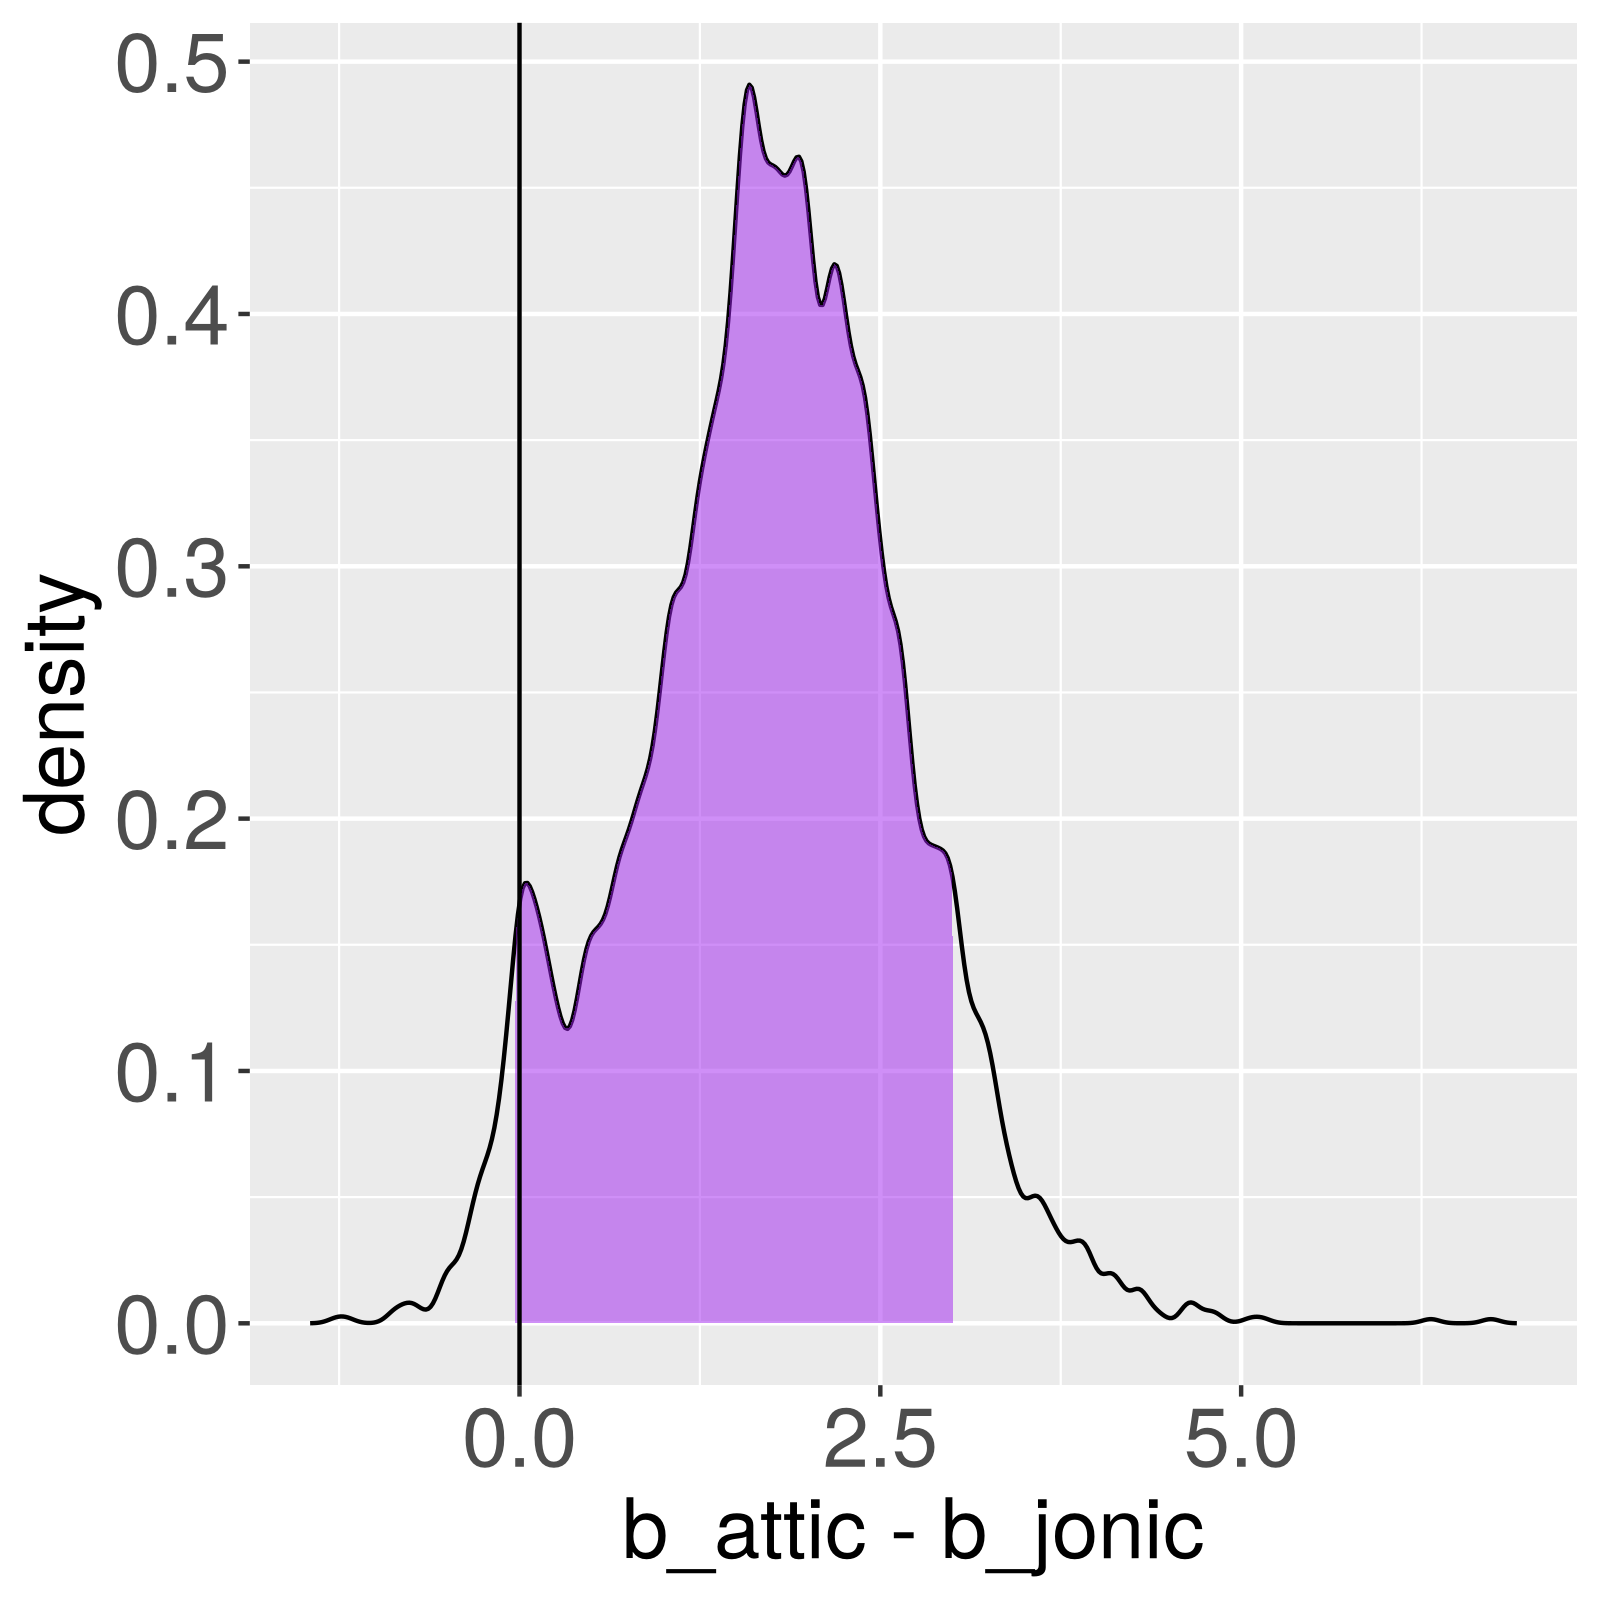
\includegraphics[width=0.5\linewidth]{./plots/posterior_diff_dia.png}
\end{figure}

O efeito direto estimado de autoria, isto é dos diversos fatores não observados
do idioleto e socioleto dos autores a quem os textos foram atribuídos, é
bastante disperso, tanto entre autores (\emph{vide} o valor de
$\sigma_\text{Autor}$) quanto dentro de um mesmo autor (notar o desvio padrão
moderado em todos os autores).
É particularmente notável que a estimativa para Heródoto, cujo \emph{corpus}
contribui com um número razoável de exemplos, é a mais incerta
($\sigma_{\text{Herodotus}} \simeq 0.55$).

\begin{figure}[!b]
  \begin{center}
    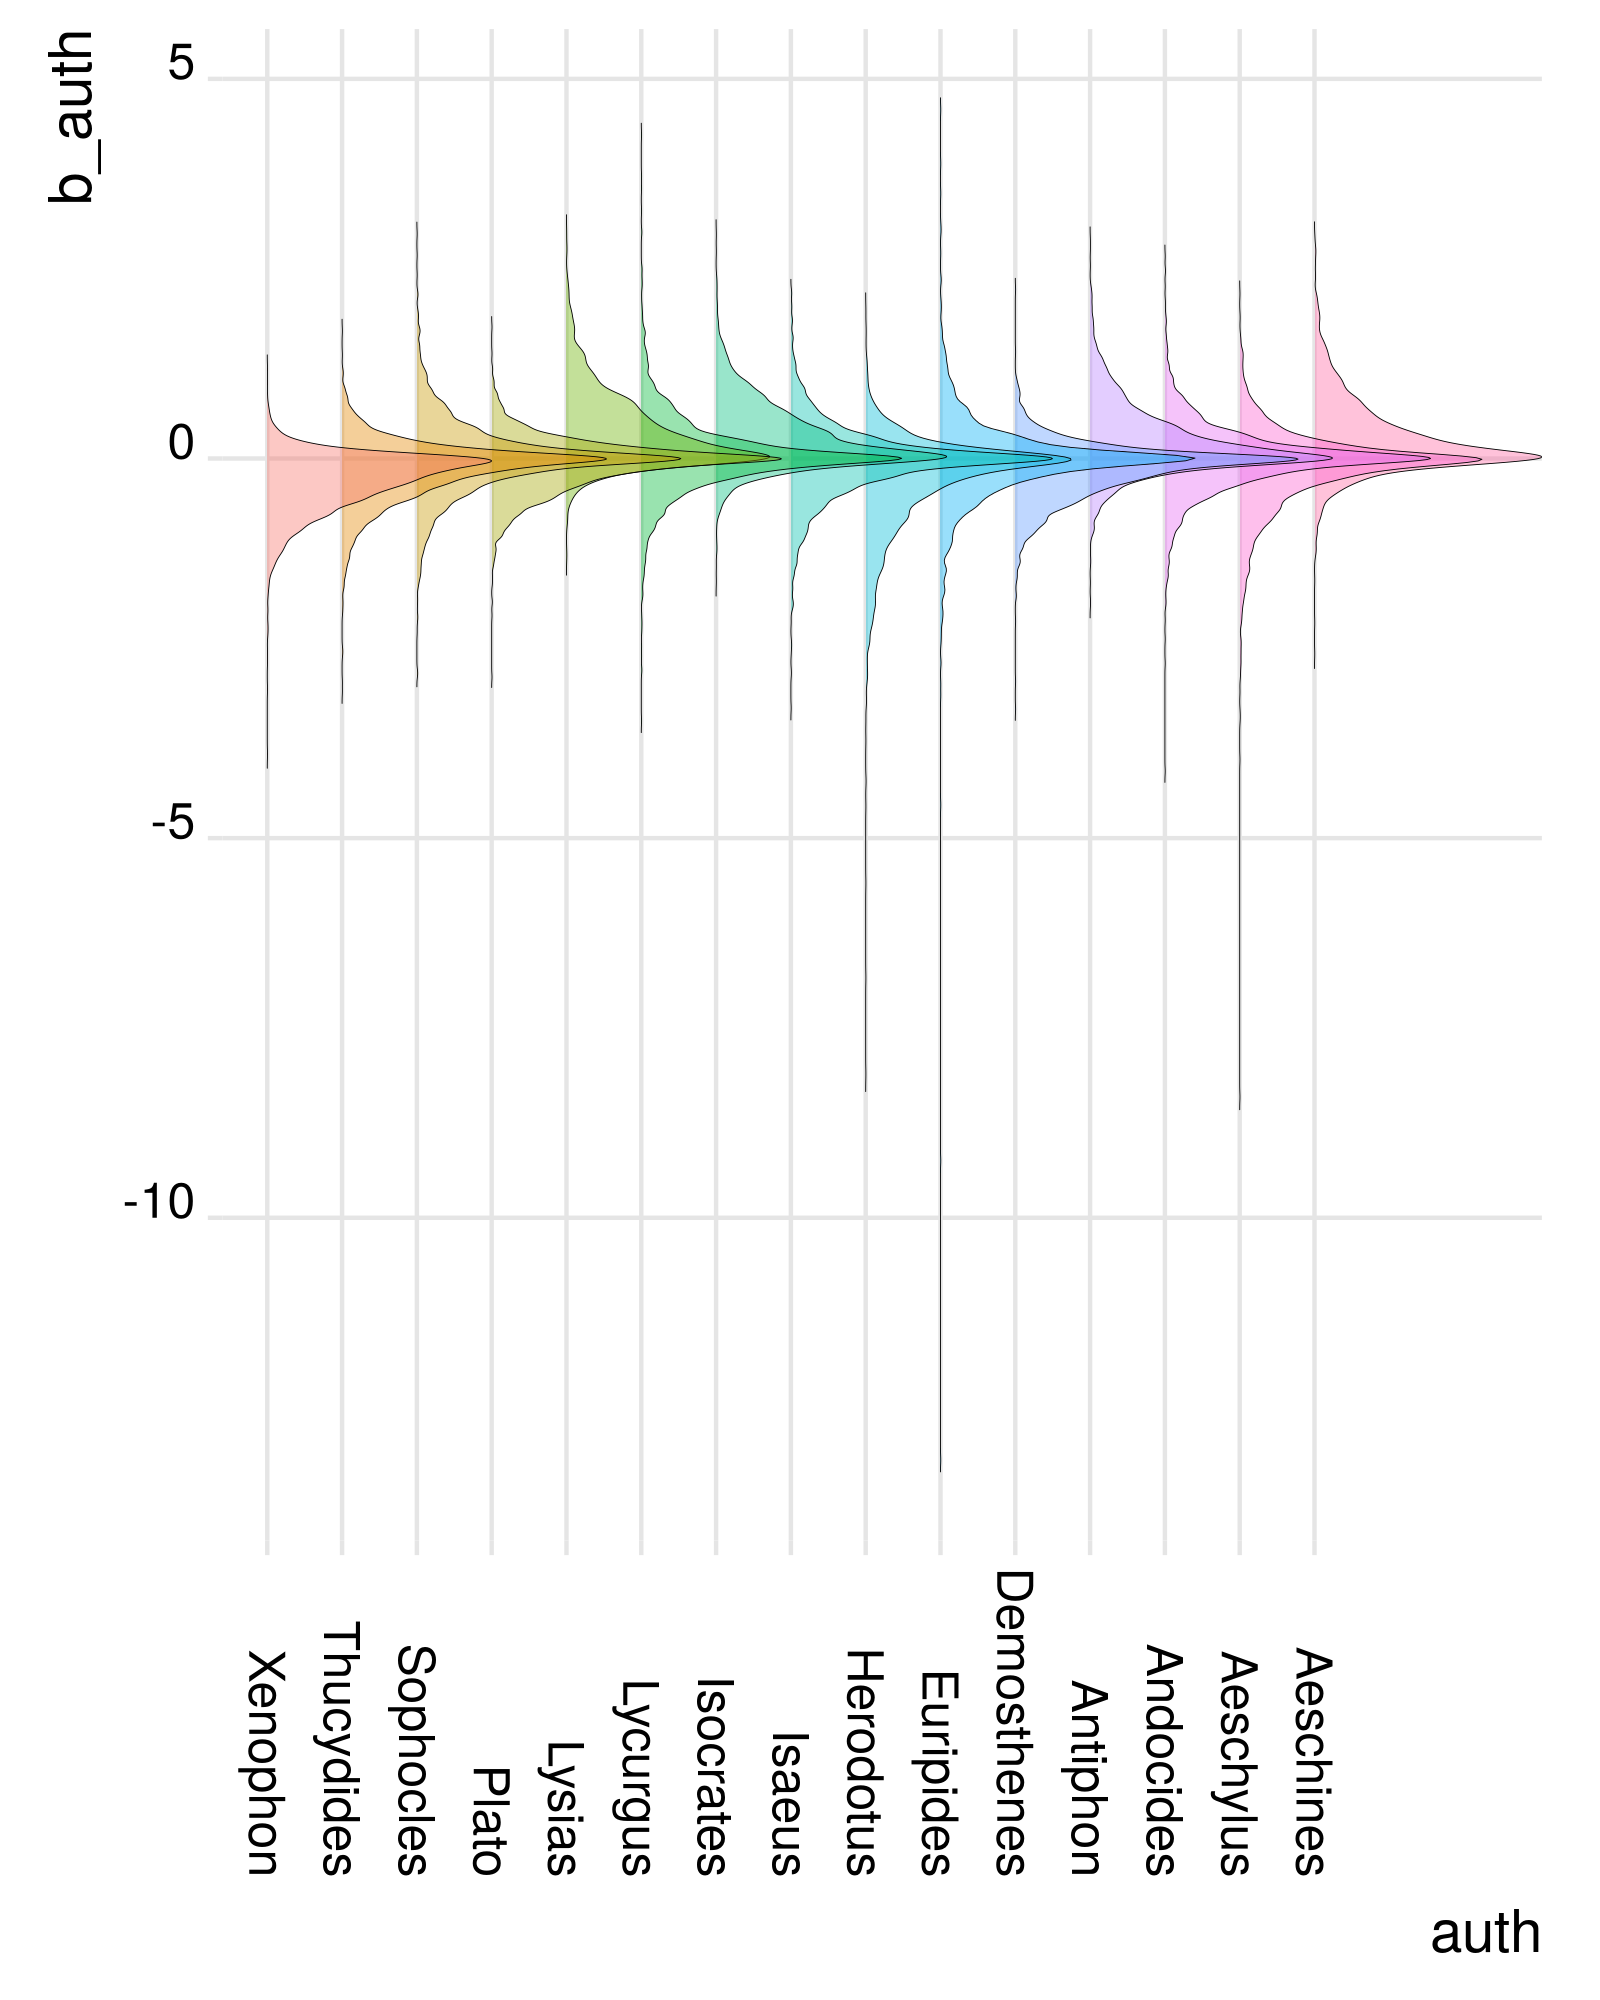
\includegraphics[width=0.75\linewidth,angle=90]{./plots/rainbow_author.png}
  \end{center}
\end{figure}

% section Authorship and Dialect (end)

% chapter Analysis (end)


\end{document}
